\documentclass[11pt, xcolor={dvipsnames, svgnames, table, x11names}, color]{beamer}

\usepackage{amsmath, amssymb, amsthm, amsfonts, mathtools}
\usepackage{graphicx}
\usepackage{physics, qcircuit}

\newcommand{\I}{\mathbb{I}}
\newcommand{\R}{\mathbb{R}}
\newcommand{\F}{\mathbb{F}}

\renewcommand{\H}{\mathcal{H}}

\newcommand{\OH}{\hat{H}}
% \usepackage{dracula-beamer}

\usetheme{Boadilla}
\usecolortheme{seahorse}
\usefonttheme{structurebold}
\setbeamercovered{invisible}
% \beamertemplatenavigationsymbolsempty

\title{Random Quantum Circuits}
\subtitle{A Glimpse into Quantum Randomness}
\author[Piyush Kumar Singh]{Piyush Kumar Singh\inst{1} \and Dr.~Sambuddha Sanyal\inst{2}}
\institute[22MS027]{
    \inst{1}%
    % 22MS027\\
    Department of Physical Sciences\\
    IISER Kolkata
    \and
    \inst{2}%
    Department of Physical Sciences\\
    IISER Tirupati
    \and
    NIUS Physics (Camp 20)
}
\date{September 1, 2024}

\begin{document}


\begin{frame}
    \titlepage
\end{frame}


\begin{frame}
    \frametitle{Outline}
    \tableofcontents
\end{frame}


\section{Introduction}
\begin{frame}
    \frametitle{Introduction}
\end{frame}


\section{Preliminaries}
\begin{frame}
    \frametitle{Preliminaries}
    For the sake of completeness, we will briefly go through some of the basic concepts that will be used in the subsequent sections.

    We will cover the following topics:
    \begin{itemize}
        \item Linear Algebra
              \begin{itemize}
                  \item Tensor Products
              \end{itemize}
        \item Group Theory
              \begin{itemize}
                  \item Unitary Group (Special emphasis on Haar Random Unitaries)\\
                        A bit of \alert{measure theory} on the way.
              \end{itemize}
        \item Quantum Mechanics
              \begin{itemize}
                  \item Measurements vs Projective Measurements
              \end{itemize}
    \end{itemize}
\end{frame}


\subsection{Linear Algebra}
\begin{frame}
    % \frametitle{Preliminaries}
    \frametitle{Linear Algebra: Basic Concepts}
    Assuming that the audience is familiar with basic linear algebra concepts like
    \begin{itemize}
        \item Hermitian and Unitary matrices
              \only<2>{
                  \begin{alignat*}{2}
                      H^\dag   & = H           \qquad & \quad \text{Hermitian} \\
                      U^\dag U & = UU^\dag = I \qquad & \quad \text{Unitary}
                  \end{alignat*}
              }
        \item Eigenvalues and eigenvectors
              \only<3>{
                  \begin{equation*}
                      A\ket{\psi} = \lambda\ket{\psi}
                  \end{equation*}
              }
        \item Inner product and outer product
              \only<4>{
                  \begin{alignat*}{2}
                      \ip{\cdot}{\cdot} : V \times V & \to \mathbb{C} \qquad     & \quad \text{Inner Product} \\
                      \op{\cdot}{\cdot} : V \times V & \to \mathcal{L}(V) \qquad & \quad \text{Outer Product}
                  \end{alignat*}
              }
        \item Diagonalization of matrices
              \only<5>{
                  \begin{equation*}
                      A = PDP^{-1} \quad \text{where} \quad D = \mqty(\dmat{\lambda_1, \lambda_2, \ddots, \lambda_n})
                  \end{equation*}
              }
        \item Matrix exponentiation
              \only<6>{
                  \begin{equation*}
                      e^{A} = \I + A + \frac{A^2}{2!} + \cdots
                  \end{equation*}

              }
              \only<7>{
                  \begin{gather*}
                      \intertext{If $A$ is diagonalizable, then}
                      e^{A} = Pe^{D}P^{-1} \quad \text{where} \quad e^{D} = \mqty(\dmat{e^{\lambda_1}, e^{\lambda_2}, \ddots, e^{\lambda_n}})
                  \end{gather*}
              }
    \end{itemize}
\end{frame}

\begin{frame}
    \frametitle{Linear Algebra: Tensor Products}
    \begin{definition}[Tensor Product]
        Let $V$ and $W$ be vector spaces over a field $\F$. The tensor product of $V$ and $W$, denoted by $V \otimes W$, is a vector space over $\F$ with the following properties:
        \begin{enumerate}
            \item For any $v \in V$ and $w \in W$, $v \otimes w \in V \otimes W$.
            \item The tensor product is bilinear, i.e., for any $v, v' \in V$, $w, w' \in W$, and $a, b \in \F$,
                  \begin{equation*}
                      (a v + b v') \otimes w = a(v \otimes w) + b(v' \otimes w)
                  \end{equation*}
                  and
                  \begin{equation*}
                      v \otimes (a w + b w') = a(v \otimes w) + b(v \otimes w')
                  \end{equation*}
        \end{enumerate}
    \end{definition}

    This gives a way to combine two vector spaces to form a new vector space. In the context of quantum mechanics, the tensor product is used to represent composite systems.
\end{frame}


\subsection{Measure Theory}
\begin{frame}
    \frametitle{Measure Theory}
    \begin{definition}[Measure of a Set]
        Let $\mathcal{A}$ be a \alert{$\sigma$-algebra} on a set $X$. A function $\mu: \mathcal{A} \to [0, \infty]$ is called a measure on $\mathcal{A}$ if it satisfies the following properties:
        \begin{enumerate}
            \item $\mu(\emptyset) = 0$.
            \item Countable additivity: For any countable collection of pairwise disjoint sets $\qty{A_i}_{i \in \mathbb{N}} \subset \mathcal{A}$,
                  \begin{equation*}
                      \mu\qty(\bigcup_{i \in \mathbb{N}} A_i) = \sum_{i \in \mathbb{N}} \mu(A_i).
                  \end{equation*}
        \end{enumerate}
    \end{definition}

    \begin{example}[Lebesgue Measure]
        For any interval $I = [a, b] \subset \R$, the Lebesgue measure $\mu(I) = b - a$.
    \end{example}
\end{frame}

\begin{frame}
    \frametitle{Measure Theory: Translation Invariance}
    \begin{definition}[Translation Invarianct Measure]
        A measure $\mu$ on a $\sigma$-algebra $\mathcal{A}$ is said to be translation invariant if for all $A \in \mathcal{A}$ and $x \in X$, $\mu(A) = \mu(A + x)$.
    \end{definition}

    \begin{example}[Lebesgue Measure]
        For any interval $I = [a, b] \subset \R$, and $x \in \R$, the Lebesgue measure $\mu(I) = \mu(I + x) = b - a$. Thus, the Lebesgue measure is translation invariant.
    \end{example}

    \onslide<2->{
        We are particularly interested in translation invariant measures on a set $X$ as they allow us to define a notion of uniformity on $X$.

        A translation-invariant measure would ensure that every region of the space is treated equally, regardless of its position.
    }
\end{frame}

\subsection{Group Theory}
\begin{frame}
    \frametitle{Group Theory}
    \begin{definition}[Group]
        A group is a set $G$ along with a binary operation $*$ such that the following properties are satisfied:
        \begin{enumerate}
            \item Closure: For all $a, b \in G$, $a * b \in G$.
            \item Associativity: For all $a, b, c \in G$, $(a * b) * c = a * (b * c)$.
            \item Identity: There exists an element $e \in G$ such that for all $a \in G$, $a * e = e * a = a$.
            \item Inverse: For all $a \in G$, there exists an element $a^{-1} \in G$ such that $a * a^{-1} = a^{-1} * a = e$.
        \end{enumerate}
    \end{definition}
    \begin{example}<2>[General Linear Group]
        The set of all $n \times n$ invertible matrices with matrix multiplication as the binary operation forms a group called the General Linear Group, denoted by $\text{GL}(n, \mathbb{C})$.
    \end{example}
\end{frame}

\begin{frame}
    \frametitle{Group Theory: Unitary Group}
    There is a specific subgroup of the General Linear Group that is of particular interest to us i.e., the Unitary Group.
    \begin{definition}[Unitary Group]
        The unitary group $\text{U}(n)$ is the group of all $n \times n$ unitary matrices.
    \end{definition}
    \begin{example}[Special Unitary Group]
        The set of all $n \times n$ unitary matrices with determinant $1$ forms a subgroup of the unitary group called the Special Unitary Group, denoted by $\text{SU}(n)$.
    \end{example}
\end{frame}

\begin{frame}
    \frametitle{Group Theory: Haar Random Unitaries}
    Since we are interested in constructing random quantum circuits, we need a way to generate random unitaries uniformly from the unitary group. This is where Haar measure comes into play.
    \begin{definition}[Haar Measure]
        Let $(G, \cdot)$ be a \alert{locally compact topological group}. A Haar measure $\mu$ on $G$ is a translation-invariant measure that is non-zero on open sets.
    \end{definition}

    In case of the unitary group, the Haar measure of the unitary group is finite, thus allowing us to define a \alert{probability distribution} on the unitary group. Since the Haar measure is translation invariant, it ensures that the generated unitaries are uniformly distributed over the unitary group.
\end{frame}

\section{Quantum Mechanics}
\begin{frame}
    \frametitle{Quantum Mechanics}
    Using Dirac Notation, we can write Schr\"odinger equation as
    \begin{equation*}
        i \hbar \dv{\ket{\Psi}}{t} = \OH \ket{\Psi} ~ \implies ~ \ket{\Psi; t} = \mathcal{U}_t \ket{\Psi; 0},
    \end{equation*}
    where $\mathcal{U}_t := \exp(\flatfrac{-i \OH t}{\hbar})$ is the time-evolution operator. Since Hamiltonian is hermitian, then by definition time-evolution operator is unitary.

    \begin{alertblock}{Why Unitary Operators?}
        This identification implies that to study the dynamics of a quantum system evolving under a random Hamiltonian, we can employ random unitaries rather than solving the Schr\"odinger equation.
    \end{alertblock}
\end{frame}

\subsection{Projective Measurements}
\begin{frame}
    \frametitle{Quantum Mechanics: Projective Measurements}
    \begin{definition}[Projective Measurement]

    \end{definition}
\end{frame}


\section{Circuit Structure}
\begin{frame}
    \frametitle{Circuit Structure}
    \begin{figure}[H]
        \[
            \Qcircuit @C=1em @R=1em {
            & \lstick{1} & \multigate{1}{u_{1,1}} & \qw & \multigate{1}{u_{3,1}} & \qw & \multigate{1}{u_{5,1}} & \qw & \rstick{\cdots}\qw  \\
            & \lstick{2} & \ghost{u_{1,1}}        & \multigate{1}{u_{2,2}} & \ghost{u_{3,1}}        & \multigate{1}{u_{4,2}} & \ghost{u_{5,1}}        & \multigate{1}{u_{6,2}} & \rstick{\cdots}\qw  \\
            & \lstick{3} & \multigate{1}{u_{1,3}} & \ghost{u_{2,2}} & \multigate{1}{u_{3,3}} & \ghost{u_{4,2}} & \multigate{1}{u_{5,3}} & \ghost{u_{6,2}} & \rstick{\cdots}\qw  \\
            & \lstick{4} & \ghost{u_{1,3}}        & \multigate{1}{u_{2,4}} & \ghost{u_{3,3}}        & \multigate{1}{u_{4,4}} & \ghost{u_{5,3}}        & \multigate{1}{u_{6,4}} & \rstick{\cdots}\qw  \\
            & \lstick{5} & \multigate{1}{u_{1,5}} & \ghost{u_{2,4}} & \multigate{1}{u_{3,5}} & \ghost{u_{4,4}} & \multigate{1}{u_{5,5}} & \ghost{u_{6,4}} & \rstick{\cdots}\qw  \\
            & \lstick{6} & \ghost{u_{1,5}}        & \multigate{1}{u_{2,6}} & \ghost{u_{3,5}}        & \multigate{1}{u_{4,6}} & \ghost{u_{5,5}}        & \multigate{1}{u_{6,6}} & \rstick{\cdots}\qw  \\
            & \lstick{7} & \multigate{1}{u_{1,7}} & \ghost{u_{2,6}} & \multigate{1}{u_{3,7}} & \ghost{u_{4,6}} & \multigate{1}{u_{5,7}} & \ghost{u_{6,6}} & \rstick{\cdots}\qw  \\
            & \lstick{8} & \ghost{u_{1,7}}        & \qw & \ghost{u_{3,7}}        & \qw & \ghost{u_{5,7}}        & \qw & \rstick{\cdots}\qw
            }
        \]
        \caption{A spacetime diagram of 8 qubits RQC. This arrangement of two-site unitary gates will be called a brickwork structure.}
        \label{fig:brickwork}
    \end{figure}
\end{frame}

\begin{frame}
    \frametitle{State Trajectory}
    \begin{figure}[H]
        \centering
        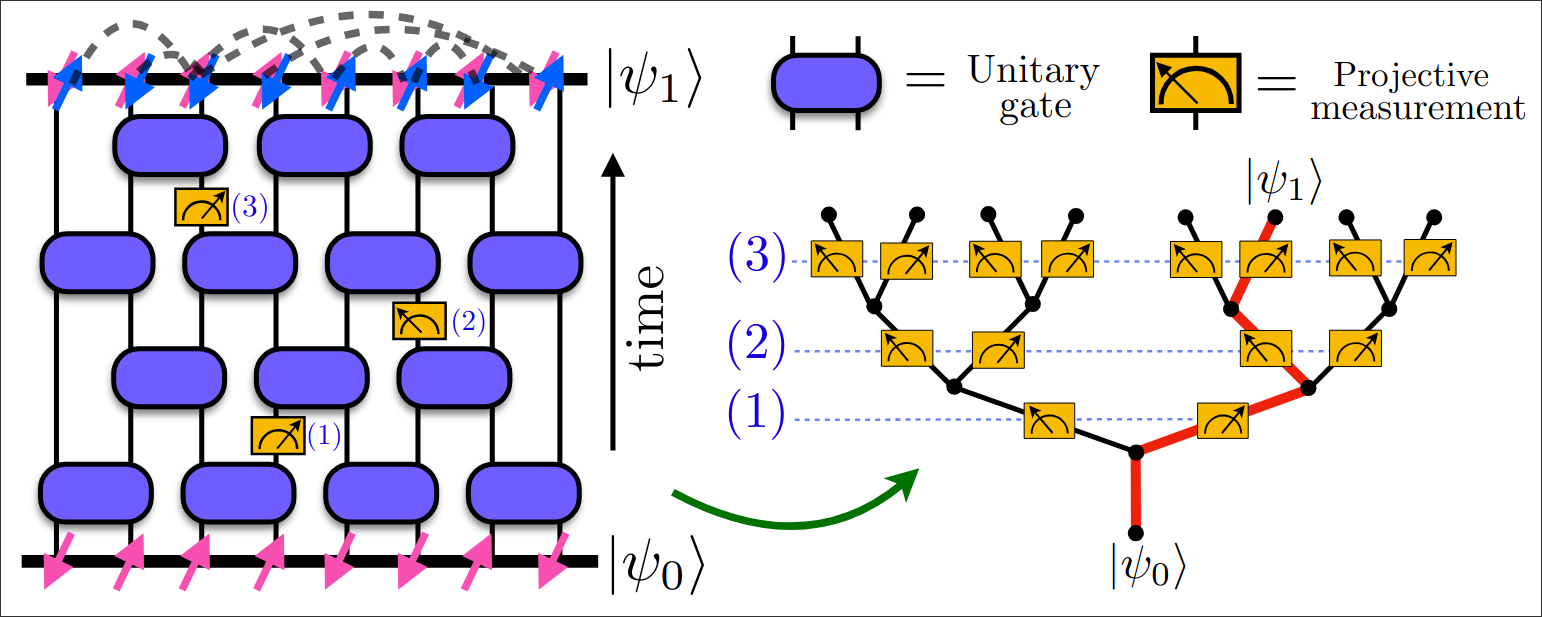
\includegraphics[width=\textwidth]{images/spacetime-brickwork.png}
        \caption{Hello}
        \label{fig:Trajectory}
    \end{figure}
\end{frame}


\section{Fidelity}
\begin{frame}
    \frametitle{Fidelity}
    \begin{definition}[Fidelity]
        Fidelity measures “overlap” between two states from a given Hilbert space $\H$. Consider two states $\ket{\Psi}$ and $\ket{\Phi}$, the fidelity between them is defined as
        \begin{equation*}
            F(\ket{\Psi}, \ket{\Phi}) = \abs{\ip{\Psi}{\Phi}}^2.
        \end{equation*}
    \end{definition}


\end{frame}


\section{Operator Spread}
\begin{frame}
    \frametitle{Operator Spread}
\end{frame}


\section{Anderson Chain}
\begin{frame}
    \frametitle{Anderson Chain}
\end{frame}


\begin{frame}
    \begin{center}
        \Huge{Thank You!}
    \end{center}
\end{frame}


\end{document}
